\scanpage{15}
Quelles conditions faut-il imposer à a) b) c)
pour que ces données proviennent d'un
polygône régulier? Signalons condition (6),
\figure{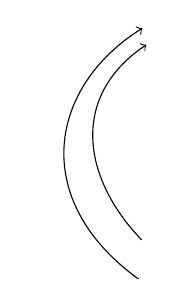
\begin{tikzpicture}[x=1cm,y=.7cm]
\draw[->] (.88,0).. controls (-.52,1.45) and (-.25,3.50)..(.93,4.55);
\draw[->] (.92,.71).. controls (.16,1.84) and (.01,3.32)..(.98,4.25);
\end{tikzpicture}}
% Both conditions are carried upward in the left margin; the written rows run (9), (8), (7).
\[
\inserted{\Gamma^{\unsure{0|\circ}}\ \text{fini}}\tag*{(7)}
\]
\[
\inserted{S\ \text{est un torseur sous }\Gamma^0}\tag*{(8)}
\]
et ensuite
\[
\deleted{\unsure{(7)|\text{et}}}\quad
\deleted{\unsure{\operatorname{card} S|\text{condition}}}\,
\left\{\begin{aligned}&S\ \text{n'est pas contenu ds une}\\&\text{droite de }E\end{aligned}\right.
\tag*{(9)}
\]
Ces \deleted{quatre} \deleted{\unsure{(6) à (9)}} conditions \inserted{(6 à 9)} suffisent, car la
structure de torseur sur $S$ sous $\Gamma^0$
met sur $S$ (grâce à $\omega\subset\Gamma^0$ \inserted{\unsure{et (7-)|et (7)}}) une
structure de $n$-polygone combinatoire
($n=\operatorname{card}\Gamma^0$) \inserted{-- on utilise (9) pour avoir $\Gamma\hookrightarrow\deleted{\operatorname{Aut}}\unsure{\mathfrak S|\circlearrowright}_S$ d'où $\omega\simeq\omega'\subset\mathfrak S_S$}\,;
\deleted{et si $\sigma\in\Gamma$ est comme ds (6), il induit un autom de $(S,\omega)$ qui renverse l'orientation, donc $\Gamma$ induit \unsure{et induit} \unsure{pas|pour} exactement le groupe des autom de}
$\Gamma'$ est son grpe des autom, on a évidemt
\diagram{\begin{tikzcd}[ampersand replacement=\&,column sep=small,row sep=0em]
\Gamma\arrow[r,hook,"\unsure{\sim|\omega}"]\&\Gamma'\\[-2pt]
\rotatebox{90}{$\subset$}\&\rotatebox{90}{$\subset$}\\[-2pt]
\Gamma^0\arrow[r,phantom,"\simeq"]\&\Gamma'{}^0
\end{tikzcd}}
qui induit un \uline{isom}orph.

Si on a \unsure{fixé|fixer|fixe} $n$, (7) devient.
\[
\operatorname{card}\Gamma^0\simeq\mathbb{Z}/n\mathbb{Z}.\tag*{$(7')$}
\]
% archive sheet number: 14

